\begin{frame}
\begin{center}
  \LARGE Heuristic: Hamiltonian Path
\end{center}
\end{frame}

%\begin{frame}
%\frametitle{Hamiltonian Path Initial Solution}
%\begin{itemize}
%	\item Start at the Tower
%	\item Use nearest neighbor heuristic
%	\item Append vertex to path
%	\item Insert vertex 
%\end{itemize}
%\end{frame}
%\begin{frame}
%\frametitle{Hamilton Path Initial}
%\begin{adjustbox}{max width=0.9\paperwidth,center}
%	\begin{tikzpicture}[node distance=3cm]
%	\tikzstyle{vertex}=[draw,shape=circle, minimum size=1cm];
%	\node[vertex] (1){1};
%	\node[node distance=0.5cm] (left) [left= of 1]{};
%	\node[vertex] (2) [right=of 1] {2};
%	\node[vertex] (3) [right=of 2] {3};
%	\coordinate (center) at ($(1)!0.5!(2)$);
%	\node[vertex] (v) [below=1cm of center] {v};
%	\node[vertex] (w) [right=of 3] {w};
%	
%	\draw[line width=0.55mm,black] (1) -- (2);
%	\draw[line width=0.55mm,black] (2) -- (3);
%	\draw[line width=0.55mm,black] (1) -- (left);
%	\end{tikzpicture}
%\end{adjustbox}
%\end{frame}

\begin{frame}
\frametitle{Initial Solution: Hamiltonian Path}
\large i) Append
\vspace{5pt}

\begin{adjustbox}{max width=0.9\paperwidth,center}
	\begin{tikzpicture}[node distance=3cm]
	\tikzstyle{vertex}=[draw,shape=circle, fill, inner sep=0pt, minimum size=0.25cm];
	\node[vertex] (1){1};
	\node[node distance=0.5cm] (left) [left= of 1]{};
	\node[vertex] (2) [right=of 1] {2};
	\node[vertex] (3) [right=of 2] {3};
	\coordinate (center) at ($(1)!0.5!(2)$);
	\node[vertex] (v) [below=1cm of center] {v};
	\node[vertex] (w) [right=of 3] {w};
	\node (legend1) [above=0.9cm of w]{};
	\node (legend2) [left=0.5cm of legend1]{add edge};
	
	\draw[line width=0.55mm,blue, dashed] (legend1) -- (legend2);
	
	\draw[line width=0.55mm,black] (1) -- (2);
	\draw[line width=0.55mm,black] (2) -- (3);
	\draw[line width=0.55mm, dashed, blue] (3) -- (w);
	\draw[line width=0.55mm,black] (1) -- (left);
	\end{tikzpicture}
\end{adjustbox}%

\noindent\makebox[\linewidth]{\rule{\paperwidth}{3pt}}
\vspace{5pt}
\large ii) Insert
\vspace{5pt}

\begin{adjustbox}{max width=0.9\paperwidth,center}
	\begin{tikzpicture}[node distance=3cm]
	\tikzstyle{vertex}=[draw,shape=circle, fill, inner sep=0pt, minimum size=0.25cm];
	\node[vertex] (1){1};
	\node[node distance=0.5cm] (left) [left= of 1]{};
	\node[vertex] (2) [right=of 1] {2};
	\node[vertex] (3) [right=of 2] {3};
	\coordinate (center) at ($(1)!0.5!(2)$);
	\node[vertex] (v) [below=1cm of center] {v};
	\node[vertex] (w) [right=of 3] {w};
	
	\draw[line width=0.55mm,black] (1) -- node[strike out,draw, red]{} (2);
	\draw[line width=0.55mm,black] (2) -- (3);
	\draw[line width=0.55mm, dashed, blue] (1) -- (v);
	\draw[line width=0.55mm, dashed, blue] (2) -- (v);
	\draw[line width=0.55mm,black] (1) -- (left);
	\end{tikzpicture}
\end{adjustbox}
\end{frame}


%\begin{frame}
%\frametitle{Local Search: Hamiltonian Path -- Triangulation}
%\begin{itemize}
%	\item For each edge and vertex we can 
%	\item x
%	\item z
%\end{itemize}
%\end{frame}
\begin{frame}
\frametitle{Local Search: Hamiltonian Path -- Triangulation}


\begin{figure}
	\begin{adjustbox}{max width=0.9\paperwidth,center}
	\begin{tikzpicture}[node distance=3cm]
	\tikzstyle{vertex}=[draw,shape=circle, minimum size=1cm];
	
	\node[vertex] (w) {w};
	\node[vertex] (v) [below=3cm of w] {v};
	\coordinate (center) at ($(w)!0.5!(v)$);
	\node[vertex] (i) [right=2cm of center] {x};
	\node[vertex] (i+) [above right=0.5cm and 4cm of i] {y};
	\node[vertex] (i-) [below right=0.5cm and 4cm of i] {z};
	\node[node distance=0.5cm] (up) [above= of w]{};
	\node[node distance=0.5cm] (down) [below= of v]{};
	\node[node distance=0.5cm] (up_i) [above= of i+]{};
	\node[node distance=0.5cm] (down_i) [below= of i-]{};
	
	\draw[line width=0.55mm,black] (w) -- (up);
	\draw[line width=0.55mm,black] (v) -- (down);
	\draw[line width=0.55mm,black] (i+) -- (up_i);
	\draw[line width=0.55mm,black] (i-) -- (down_i);
	
	\draw[line width=0.55mm, black] (w) -- (v);
	\draw[line width=0.55mm, black] (i) -- (i+);
	\draw[line width=0.55mm, black] (i) -- (i-);
	%\draw[line width=0.55mm, dashed, purple] (w) -- (i);
	%\draw[line width=0.55mm, dashed, purple] (v) -- (i);
	%\draw[line width=0.55mm, dashed, purple] (i+) -- (i-);
	\end{tikzpicture}
	\end{adjustbox}
	\caption{Starting point.}
\end{figure}

\end{frame}

\begin{frame}
\frametitle{Local Search: Hamiltonian Path -- Triangulation}
\begin{figure}
\begin{adjustbox}{max width=0.9\paperwidth,center}
	\begin{tikzpicture}[node distance=3cm]
	\tikzstyle{vertex}=[draw,shape=circle, minimum size=1cm];
	\node[vertex] (w) {w};
	\node[vertex] (v) [below=3cm of w] {v};
	\coordinate (center) at ($(w)!0.5!(v)$);
	\node[vertex] (i) [right=2cm of center] {x};
	\node[vertex] (i+) [above right=0.5cm and 4cm of i] {y};
	\node[vertex] (i-) [below right=0.5cm and 4cm of i] {z};
	\node (legend1) [above right=2cm and 1cm of i] {added edges};
	\node (legend2) [right=1cm of legend1] {};
	\node (l1) [above=0.1cm of legend1] {deleted edges};
	\node (l2) [right=1cm of l1] {};
	
	\node[node distance=0.5cm] (up) [above= of w]{};
	\node[node distance=0.5cm] (down) [below= of v]{};
	\node[node distance=0.5cm] (up_i) [above= of i+]{};
	\node[node distance=0.5cm] (down_i) [below= of i-]{};
	
	\draw[line width=0.55mm,blue, dashed] (legend1) -- (legend2); 
	\draw[line width=0.55mm,black] (l1) -- node[strike out,draw, red]{} (l2); 
	
	\draw[line width=0.55mm,black] (w) -- (up);
	\draw[line width=0.55mm,black] (v) -- (down);
	\draw[line width=0.55mm,black] (i+) -- (up_i);
	\draw[line width=0.55mm,black] (i-) -- (down_i);
	
	\draw[line width=0.55mm, black] (w) -- node[strike out,draw, red]{} (v);
	\draw[line width=0.55mm, black] (i) -- node[sloped, strike out,draw, red]{} (i+);
	\draw[line width=0.55mm, black] (i) -- node[sloped, strike out,draw, red]{} (i-);
	\draw[line width=0.55mm, dashed, blue] (w) -- (i);
	\draw[line width=0.55mm, dashed, blue] (v) -- (i);
	\draw[line width=0.55mm, dashed, blue] (i+) -- (i-);
	\end{tikzpicture}
\end{adjustbox}
\caption{Check costs of added and deleted edges.}
\end{figure}
\end{frame}

\begin{frame}
\frametitle{Local Search: Hamiltonian Path -- Triangulation}
\begin{figure}
\begin{adjustbox}{max width=0.9\paperwidth,center}
	\begin{tikzpicture}[node distance=3cm]
	\tikzstyle{vertex}=[draw,shape=circle, minimum size=1cm];
	\tikzstyle{cross}=[draw, shape=cross, red];
	
	\node[vertex] (w) {w};
	\node[vertex] (v) [below=3cm of w] {v};
	\coordinate (center) at ($(w)!0.5!(v)$);
	\node[vertex] (i) [right=2cm of center] {x};
	\node[vertex] (i+) [above right=0.5cm and 4cm of i] {y};
	\node[vertex] (i-) [below right=0.5cm and 4cm of i] {z};
	\node[node distance=0.5cm] (up) [above= of w]{};
	\node[node distance=0.5cm] (down) [below= of v]{};
	\node[node distance=0.5cm] (up_i) [above= of i+]{};
	\node[node distance=0.5cm] (down_i) [below= of i-]{};
	
	\draw[line width=0.55mm,black] (w) -- (up);
	\draw[line width=0.55mm,black] (v) -- (down);
	\draw[line width=0.55mm,black] (i+) -- (up_i);
	\draw[line width=0.55mm,black] (i-) -- (down_i);
	
	\draw[line width=0.55mm, black] (w) -- (i);
	\draw[line width=0.55mm, black] (v) -- (i);
	\draw[line width=0.55mm, black] (i+) -- (i-);
	\end{tikzpicture}
\end{adjustbox}
\caption{Added edges have lower costs than deleted ones.}
\end{figure}
\end{frame}


\begin{frame}{Triangulation Neighborhood Improvement}
  \begin{figure}
    \captionsetup[subfigure]{justification=centering}
    \begin{subfigure}{0.45\textwidth}
      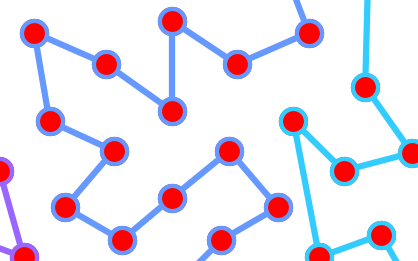
\includegraphics[width=0.75\textwidth]{./figs/init_output_hamilton_14_5_-1__SELECTION.png}
      \caption{Initial solution.}
    \end{subfigure}
    \begin{subfigure}{0.45\textwidth}
      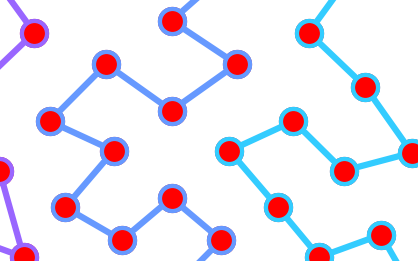
\includegraphics[width=0.75\textwidth]{./figs/output_hamilton_14_5_-1__SELECTION.png}
      \caption{After triangulation improvement.}
    \end{subfigure}
  \end{figure}
\end{frame}

\begin{frame}
  \begin{figure}
    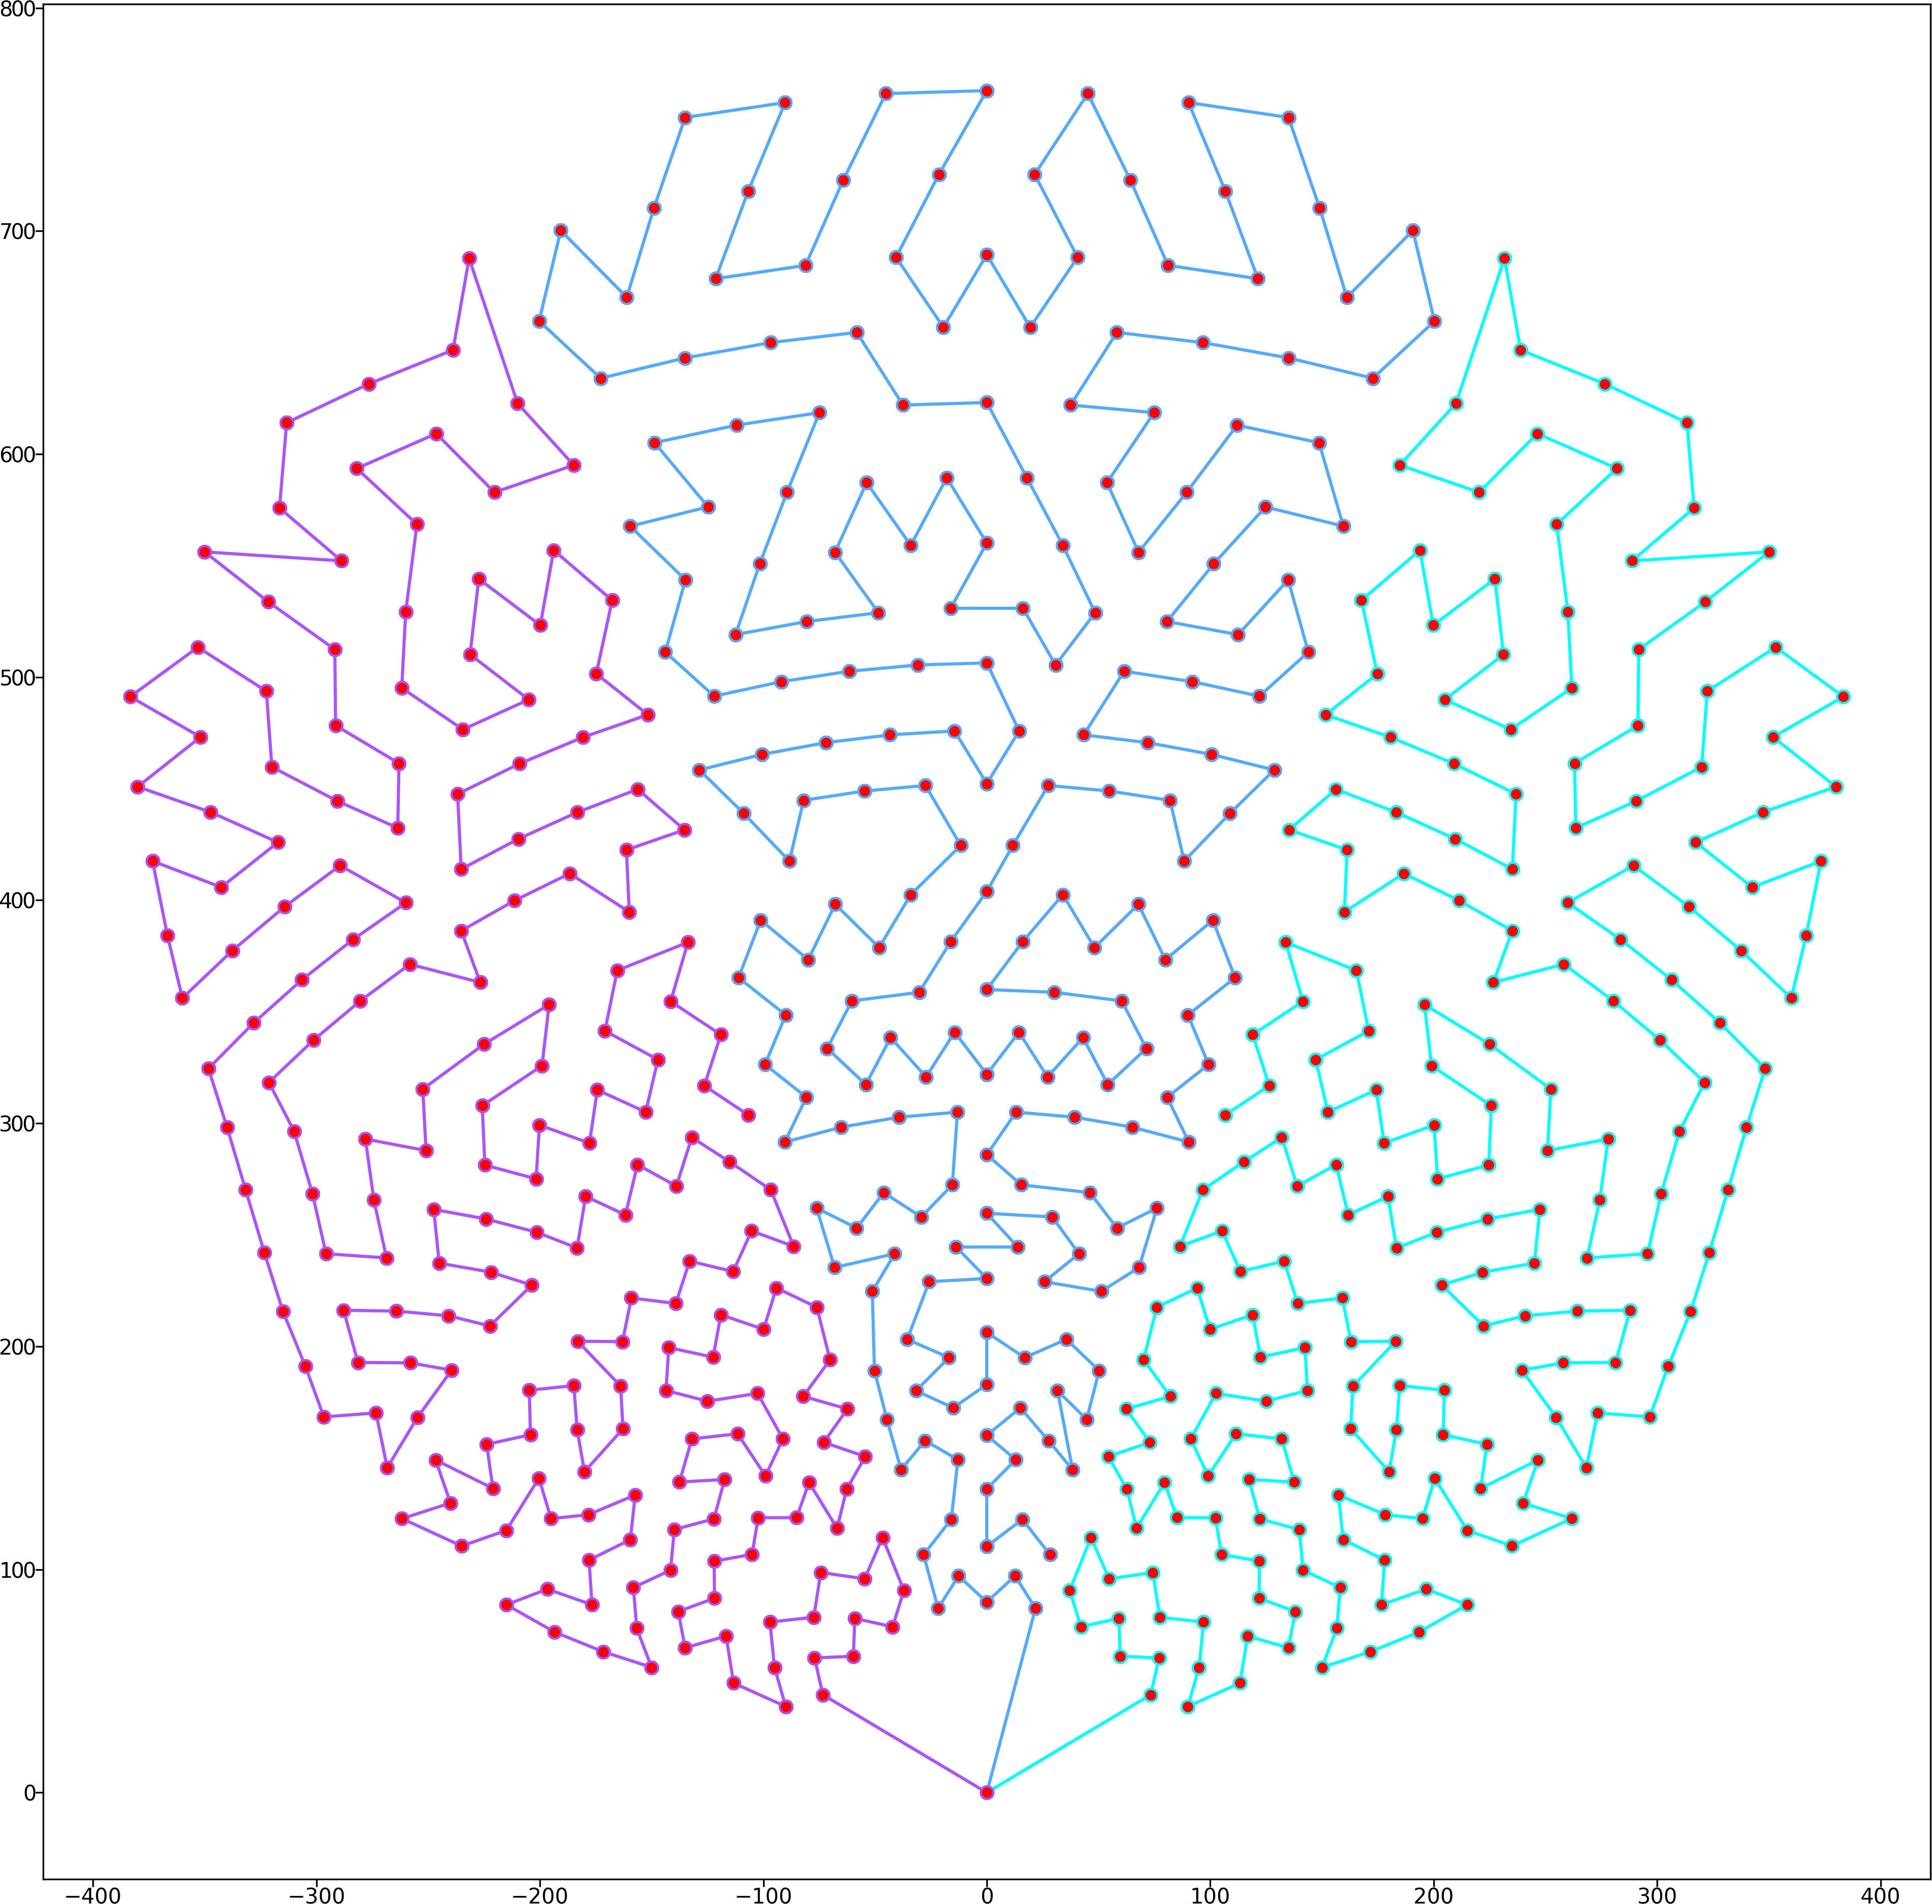
\includegraphics[width=0.72\textwidth]{./figs/hamilton_big_init.png}
    \caption{Initial Hamiltonian paths solution for 3 partitions and $54$\euro/m. Total costs: 992,324.18 \euro \ (data cables and switch costs).}
  \end{figure}
\end{frame}


\begin{frame}
  \begin{figure}
    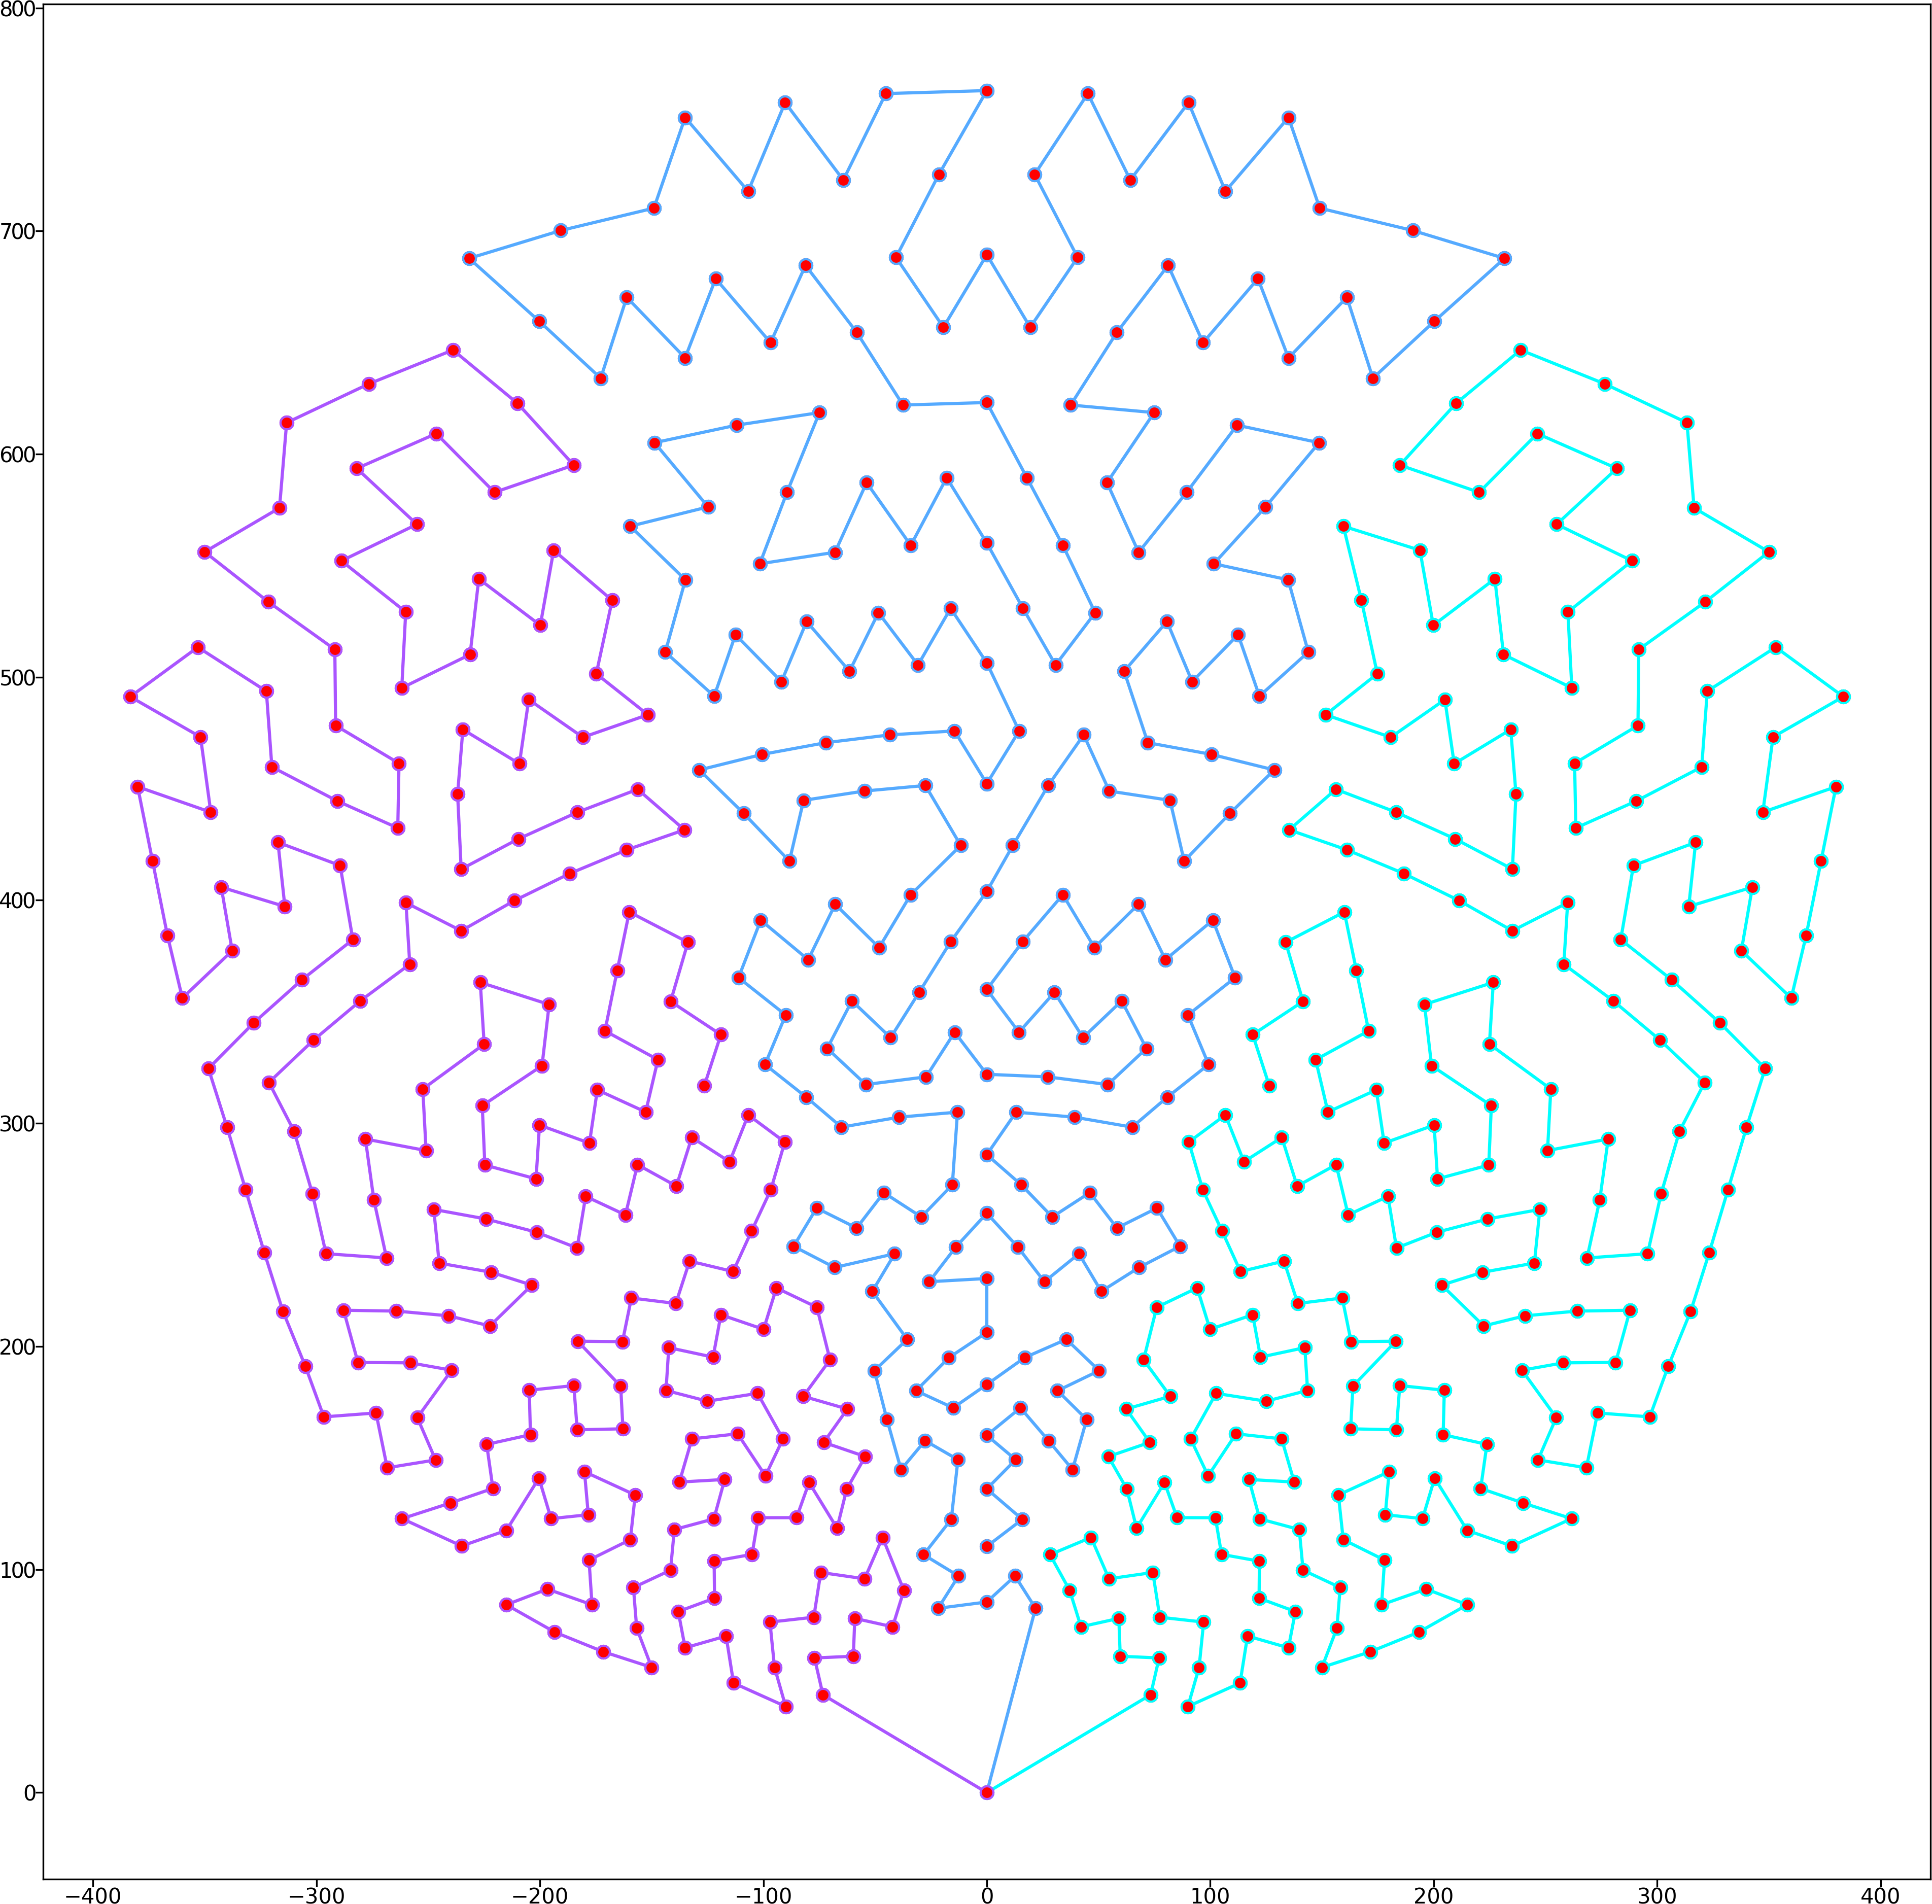
\includegraphics[width=0.72\textwidth]{./figs/hamilton_big_after_ls.png}
    \caption{After local search for Hamiltonian paths. Total costs: 971,016.47\euro.}
  \end{figure}
\end{frame}